\subsection*{A. Appetizing problem}

Дважды пытался отпроситься с пары Азат, чтобы сбегать в столовую, но преподаватель был непреклонен. Кое-как дождавшись перемены, Азат понял, что рискует не успеть проделать весь свой путь: аудитория $\rightarrow$ лифт $\rightarrow$ столовая $\rightarrow$ лифт $\rightarrow$ новая аудитория. Расстояние от любой аудитории до лифта, как и расстояние от лифта до столовой, Азат пробегает за $T$ секунд; лифт ждать не надо --- он всегда приезжает моментально; лифт движется со скоростью один этаж в секунду; ну и естественно, Азату нужно ровно $D$ секунд, чтобы покушать. Какой минимальной продолжительности должна быть перемена, чтобы Азат благополучно пообедал и не опоздал на следующую пару?

\informat{
Четыре целых числа через пробел: $N_1$, $N_2$ (от 200 до 999), $T$ и $D$ (от 1 до 1000).}

\outformat{Одно целое число --- время от выхода из аудитории $N_1$ до входа в аудиторию~$N_2$ в секундах.}

\examplee{714 601 25 300}{411}{201 201 10 10}{52}

\excomm{Аудитория с номером $N$ находится на этаже, номер которого является пер\-вой цифрой числа $N$. Например, 714 аудитория находится на седьмом этаже. Столовая находится на первом этаже.}



\subsection*{B. Bekarys' problem}

А вот Бекарыс уже покушал и готов находить четвёртые справа циф\-ры факториалов разных чисел. Ведь этим все и занимаются после плотного обеда, не так ли?

\informat{Одно целое число $N$ (от 1 до $10^{18}$).}

\outformat{Одно целое число от 0 до 9.}
 
\examplee{3}{0}{7}{5}
 
\excomm{Если в десятичной записи числа $N!$ меньше четырёх цифр, вывести ноль.}



\subsection*{С. Car showroom problem}


Да, дела у Надиры с её автосалоном идут хорошо. Правда, у него до сих пор нет названия. Надира даже частично выкупила авторские права на букву~'a'. Теперь она может использовать эту букву, но не слишком часто: ей нельзя ставить буквы~'a' рядом друг с другом. Сколько разных допустимых вариантов названий есть у Надиры?

\informat{Одно целое число $N$ от 1 до $10^7$ --- количество букв в планируемом названии автосалона.}
 
\outformat{Количество допустимых вариантов --- строк длины $N$ из строчных латинских букв, не содержащих двух букв 'a' подряд. Поскольку ответ может оказаться очень большим, его следует вывести по модулю $10^9 + 7$.}
 
\examplee{2}{675}{2017}{379347254}
 
\excomm{В первом примере допустимы все сочетания из двух букв, кроме <<aa>>.}


 
\subsection*{D. Dice problem}


Куб, находящийся во владении команды Снежный Куб и являющийся её талисманом, представляет собой кубик единичного размера. Одна его грань окрашена в красный цвет, противоположная ей --- в синий, остальные четыре белы как снег. Кубик стоит на своей красной грани в левом верхнем углу доски $N \times M$. Тимур с Еруланом (только с разрешения Александры, конечно) могут перекатить куб через ребро на одну из четырёх соседних клеток доски, если она не занята. Какое наименьшее количество перекатываний им понадобится, чтобы этот куб оказался на своей начальной позиции, стоя на синей грани?

\informat{На первой строке два целых числа $N$ и $M$ от 1 до 100. В следующих $N$ строках матрица $N$ на $M$ --- описание доски: '\#' --- недоступные клетки, '.' --- свободные клетки. Гарантируется, что клетка, на которой изначально находится кубик, свободна.}
 
\outformat{Одно целое число --- минимальное количество перекатов. Если такой по\-сле\-до\-ва\-тель\-нос\-ти перекатов не существует, вывести $-1$.}

\examplee{3 3 \newline
.\#\# \newline
...\newline
...}
{8}
{3 3 \newline
.\#\# \newline
..\#\newline
...}
{-1}

\excomm{В первом примере подходит следующая последовательность: вниз, впра\-во, впра\-во, вниз, влево, влево, вверх, вверх.}





\subsection*{E. Easy problem}


В нашем филиале чтят традиции. Вот и Куат, Димитрий и Павел переняли традицию команды Big Dipper пить чай на тренировках. Как и их старшие товарищи, они определили комфортную температуру чая, при которой его мож\-но пить --- от $L$ до $R$ градусов. Сейчас перед ними $N$ чашек с чаем. Сколько у~них различных способов смешать чай из двух чашек так, чтобы получился чай комфортной температуры?

\informat{В первой строке три целых числа: $N$ --- количество чашек, $L$ и $R$ --- границы комфортной температуры чая, где $N$ от 2 до $10^5$, $-10^9 \leqslant L \leqslant R \leqslant 10^9$ . \newline
Во второй строке $N$~целых чисел $x_i$ --- температура чая в $i$-й чашке, где $x_i$ от $-10^9$ до $10^9$.}

\outformat{Одно целое число --- количество способов получить чай нужной температуры.}
 
\examplee{
4 1 4 \newline 
1 2 3 4}
{6}
{
5 8 10 \newline
1 20 2 19 10}
{1}

\excomm{Смешивая две чашки чая с температурами $A$ и $B$, вы получите чай с тем\-пе\-ра\-ту\-рой $\dfrac{A+B}{2}$. В первом примере смешать чай можно из любых двух чашек. Во втором примере условиям удовлетворяет только одна пара (1, 19).}
 


\subsection*{F. Flat problem}

 
Плюс жизни под землёй в том, что вам не надо покупать жильё по высоким ценам, ведь вы можете вырыть себе квартиру сами! Как раз этим и занят домашний питомец Ануара --- крот Кртек. Он начинает с одной свободной квадратной клетки. Затем он выбирает одно из четырёх направлений, рас\-чи\-ща\-ет, если нужно, соседнюю клетку в этом направлении и перемещается туда. Какое максимальное количество дверей сможет поставить крот Кртек так, чтобы из любой точки полученного жилища он мог попасть в любую другую, не пройдя ни через одну дверь? 
 
\informat{Строка из не более, чем 1000 символов 'N', 'E', 'S', 'W', описывающая маршрут Кртека.}

\outformat{Ответ --- максимальное количество дверей.}

\examplee{NNNWSSSWNNN}{6}
{NNWWSSEENNWWSSEE}{1}

\excomm{Двери ставить можно только на границе двух смежных жилых клеток. В первом примере можно поставить шесть дверей следующим образом: }

\begin{center}
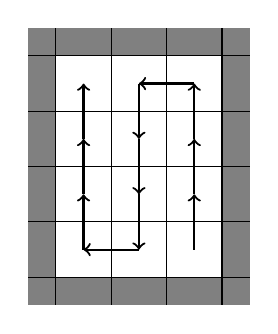
\begin{tikzpicture}[x=20,y=20]
\fill[color=gray](0.5,0.5) rectangle (4.5,5.5);
\fill[color=white](1,1) rectangle (4,5);
\draw[step=1] (0.5,0.5) grid (4.5, 5.5);

\path[->, draw, thick] (3.5, 1.5) -- (3.5, 2.5);
\path[->, draw, thick] (3.5, 2.5) -- (3.5, 3.5);
\path[->, draw, thick] (3.5, 3.5) -- (3.5, 4.5);
\path[->, draw, thick] (3.5, 4.5) -- (2.5, 4.5);
\path[->, draw, thick] (2.5, 4.5) -- (2.5, 3.5);
\path[->, draw, thick] (2.5, 3.5) -- (2.5, 2.5);
\path[->, draw, thick] (2.5, 2.5) -- (2.5, 1.5);
\path[->, draw, thick] (2.5, 1.5) -- (1.5, 1.5);
\path[->, draw, thick] (1.5, 1.5) -- (1.5, 2.5);
\path[->, draw, thick] (1.5, 2.5) -- (1.5, 3.5);
\path[->, draw, thick] (1.5, 3.5) -- (1.5, 4.5);
\end{tikzpicture}
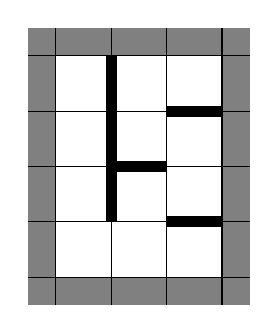
\begin{tikzpicture}[x=20,y=20]
\fill[color=gray](0.5,0.5) rectangle (4.5,5.5);
\fill[color=white](1,1) rectangle (4,5);
\draw[step=1] (0.5,0.5) grid (4.5, 5.5);

\draw[line width=4pt] (2,2) -- (2, 5);
\draw[line width=4pt] (3,3) -- (2, 3);
\draw[line width=4pt] (3,2) -- (4, 2);
\draw[line width=4pt] (3,4) -- (4, 4);
\end{tikzpicture}
\end{center}




\subsection*{G. Golden problem}


Квадрат числа 26 равен 676 --- палиндрому. Также палиндром получится, если в квадрат возвести 2285. Этими и подобными числами заинтересовался Рамазан, дав им название золотых. Все эти числа он мог бы выписать на полях Демидовича, но там слишком мало места. Каждому, кто сможет внести хоть какой-то вклад в развитие теории золотых чисел (то есть, не палиндромов, дающих палиндромы при возведении в квадрат), Рамазан обещает дать два пирожка: с картошкой и капустой. Не сто тысяч марок, конечно, но тоже до\-стой\-ная награда. Покажите, что вы заслуживаете этот приз.

\informat{В первой строке целое число $M$ от 1 до $10^5$ --- количество запросов. В следующих $M$ строках по два целых числа $L_i$, $R_i$ такие, что $1 \leqslant L_i \leqslant R_i \leqslant 10^9$.}

\outformat{$M$ строк, на каждой из которых одно целое число --- количество золотых чисел в сегменте $[L_i, R_i]$.}
 
\example{
3 \newline
2 3 \newline
22 33 \newline
222 333 
}{0 \newline
1 \newline
2
}

\excomm{Золотыми числами из третьего запроса являются 264 и 307 ($264^2=69696$, $307^2=94249$).}




\subsection*{H. Honey cake problem}


<<С понедельника никакого сладкого!>> --- твёрдо решил Илья. Но пока только суббота и перед ним на столе медовый торт. На коробке написано <<Звёздный торт>>, но Илья относится к этому названию с некоторой долей скепсиса. Всем ведь известно, что $2n$-угольный торт может называться звёздным, только если углы, от которых можно отрезать треугольный кусок, чередуются с углами, от которых нельзя отрезать треугольный кусок. Помогите Илье определить, является ли данный торт звёздным на самом деле.

 
\informat{Одно целое число $M$ от 3 до 1000 --- количество вершин торта. Далее $M$ пар целых чисел от $-1000$ до $1000$ --- координаты вершин. Вершины перечислены в порядке обхода против часовой стрелки.
}

\outformat{Если этот торт является звёздным, вывести <<YES>> (без кавычек), иначе <<NO>> (также без кавычек).}

\examplee{
8 \newline
10 0 \newline
1 1 \newline 
0 10 \newline
-1 1 \newline
-10 0 \newline
-1 -1 \newline
0 -10 \newline
1 -1
}{YES}
{
4 \newline
10 0 \newline
1 1 \newline
0 10 \newline
-10 -10
}{NO}

\excomm{На картинке видно, что торт из первого примера является звёздным. Черным цветом отмечены вершины, от которых можно отрезать треугольный кусок, белым --- от которых нельзя отрезать треугольный кусок.}

\begin{center}
\begin{tikzpicture}[x=10, y=10, every node/.style={inner sep=2pt}]
\draw 
(10,0) node [minimum size=1, shape=circle, draw, fill = black]{} -- 
(1, 1) node [minimum size=0.1, shape=circle, draw, fill = white]{} -- 
(0, 10) node [shape=circle, draw, fill = black]{} -- 
(-1, 1) node [shape=circle, draw, fill = white]{} -- 
(-10, 0) node [shape=circle, draw, fill = black]{} -- 
(-1, -1) node [shape=circle, draw, fill = white]{} -- 
(0, -10) node [shape=circle, draw, fill = black]{} -- 
(1, -1) node [shape=circle, draw, fill = white]{} --
cycle;
\end{tikzpicture}
\end{center}



\subsection*{I. Is that even a problem?}


Абырвалг. Поехали!
 
\informat{Три целых числа А, В, С от -1000 до 1000.}

\outformat{Одно целое число.}

\examplee{0 0 0}{0}{0 1 0}{1}